\documentclass[10pt,a4paper]{article}
\usepackage[T1]{fontenc}
\usepackage[utf8]{inputenc}
\usepackage[margin=25mm]{geometry}
\usepackage{lmodern}
\usepackage{microtype}
\usepackage{booktabs,tabularx}
\usepackage{xcolor}
\usepackage{tikz}
\usepackage[hidelinks]{hyperref}
\setlength{\emergencystretch}{2em}

\newif\ifdraft
\drafttrue
\newcommand{\draftnote}[1]{\ifdraft\par\smallskip\noindent
  {\small\color{gray}\textit{Draft prompt: #1}}\par\smallskip\fi}
\newcommand{\code}[1]{\texttt{\detokenize{#1}}}
\newcommand{\resultplaceholder}{\textit{To be measured}}

\title{Stack Canary Protection and PMP-Based Stack Guards in S3K}
\author{
  Agaton Pirander \and Oliver Marcusson
}
\date{
  \texttt{\{agpira, olmar\}@kth.se}\\[0.5em]
  October 2026
}

\begin{document}
\maketitle
\sloppy

\begin{abstract}
A stack buffer overflow in a C program can overwrite saved return state and
take over control flow. Process separation in a kernel such as S3K does not
prevent this, because the corruption happens inside the process. We add
compiler-generated stack canaries to the S3K kernel and its applications, and
extend them with virtualized PMP stack guards: the stack of the protected
application has no permanent memory protection entry, a trusted monitor maps
small guard-free windows on demand, and the canary and saved
\code{ra}/\code{s0} of every live frame are never mapped. An overflow
therefore faults at the first write to a guard, and the isolated monitor
suspends the application. Against an unprotected build, a 137-byte input
redirects control flow to a target function. With protection, the target is
not reached, and a write past the top of the stack is stopped by the monitor.
The main limitation is that the monitor trusts the frame events the
application sends.
\end{abstract}

\section{Introduction}
\label{sec:introduction}

Embedded and kernel software is still mostly written in C, and C does not
check array bounds. A function that copies attacker-controlled input into a
fixed-size stack buffer without a length check can write past the buffer into
the data stored above it. On RISC-V, that data includes the saved return
address \code{ra} and the saved frame pointer \code{s0}. Overwriting the saved
\code{ra} lets an attacker choose where the function returns, which is enough
to hijack control flow.

S3K is a capability-based separation kernel for RISC-V \cite{s3k}. It
isolates processes from each other with Physical Memory Protection (PMP), so
a compromised process cannot directly read or write the memory of another.
Separation does not, however, help inside a process: the overflow, the
corrupted frame and the hijacked return all happen in memory the process is
allowed to write. S3K is a useful setting for this problem because it is
small enough to change in a course project, it has no virtual memory, and its
monitor capabilities let one trusted process manage the PMP configuration of
another.

\paragraph{Research question.}
How can compiler-generated stack canaries and capability-controlled memory
protection detect and contain stack corruption in S3K, and what practical
constraints arise when implementing them?

\paragraph{Scope and contributions.}
We integrate GCC stack canaries into the S3K kernel and its user
applications, and build a vulnerable demonstration application with a
reproducible exploit. On top of the canaries we implement virtualized PMP
stack guards: a monitor process that treats the eight PMP entries of the
application like a translation lookaside buffer. It maps stack windows on
demand and never maps a guard, so that an overflow is stopped before it
overwrites anything. Individual responsibilities are described in
Section~\ref{sec:contributions}.

\section{Threat Model and Countered Vulnerabilities}
\label{sec:threat}

\subsection{Threat model}

The system consists of three S3K processes (Table~\ref{tab:processes}). The
attacker controls the input to \code{vuln} over the UART, and \code{vuln}
reads it with \code{alt_gets}, which has no bounds check. The attacker can
exploit any memory-safety bug reachable from that input. The kernel, the boot
process \code{app0} and the monitor are trusted. \code{vuln} is a benign
application that is being exploited, not a malicious program: its code is
instrumented at build time, and we assume that the frame events it sends to
the monitor are correct as long as its control flow has not been taken over.
The goal of the design is to stop the corruption before that happens.

\begin{table}[htbp]
\centering
\small
\begin{tabularx}{\linewidth}{@{}llX@{}}
\toprule
Process & PID & Role \\
\midrule
\code{app0} & 0 & Boot process. Grants memory, time, PMP, monitor and socket capabilities, then starts the monitor. Trusted. \\
\code{monitor} & 1 & Owns the guard table, maps stack windows into \code{vuln}'s PMP, classifies faults and stops \code{vuln} on an attack. Trusted. \\
\code{vuln} & 2 & Instrumented application with the unsafe \code{alt_gets} call. Sends frame events and faults to the monitor. Untrusted input. \\
\bottomrule
\end{tabularx}
\caption{Processes in the \code{projects/canaries} system.}
\label{tab:processes}
\end{table}

\subsection{Countered vulnerabilities}

The design targets stack-based memory corruption in \code{vuln}:
\begin{itemize}
  \item \emph{Linear stack-buffer overflow} into the canary and the saved
  \code{ra}/\code{s0}, the classic control-flow hijack.
  \item \emph{Non-linear writes} that skip the canary, such as an indexed
  write, and hit the saved return state directly.
  \item \emph{Canary disclosure}, where the attacker reads the canary and
  writes the correct value back while overwriting \code{ra}.
  \item \emph{Overflows through a pointer} to a buffer in a frame further up
  the call chain.
  \item \emph{Code injection on the stack}, where the payload itself is
  executed.
  \item \emph{Stack exhaustion}, where the stack grows past its bounds.
\end{itemize}

\subsection{Non-goals}

The design does not protect data-only attacks that stay inside a single frame
and never touch a guard, such as overwriting a neighbouring local variable.
It does not protect memory outside the stack, such as the heap, \code{.data}
or \code{.bss}. Kernel and hardware attacks, side channels and denial of
service are out of scope.

\section{Background}
\label{sec:background}

S3K runs on RISC-V and uses capabilities for every resource: memory ranges,
time slices, IPC channels and sockets, and \emph{monitor} capabilities that
let one process suspend, resume and reconfigure another. A memory capability
can be turned into a PMP capability and loaded into one of the process's
hardware PMP entries. On our platforms (\code{qemu_virt}) each process has
\code{S3K_PMP_CNT}~$=8$ entries. S3K PMP capabilities use NAPOT encoding, so
every region is a power of two in size and aligned to its size, with a
minimum of 8 bytes. A user-mode access that matches no PMP entry raises an
access fault, which S3K delegates to the process's own trap handler.

GCC's \code{-fstack-protector-strong} instruments every function that has a
local array or a local whose address is taken. The prologue copies the global
\code{__stack_chk_guard} into the frame, between the local buffers and the
saved registers. The epilogue compares the copy with the global value and
calls \code{__stack_chk_fail} if they differ. A canary detects a linear
overwrite only when the function returns, after the damage is done.

On systems with virtual memory, a guard page is an unmapped page next to a
protected region, so that any access to it faults. S3K has no page tables and
only eight PMP entries, far too few to give every stack frame its own guard.
Our design solves this by using the PMP entries as a cache over a complete
guard table kept in software, in the same way that a translation lookaside
buffer caches a page table.

\draftnote{Keep the next paragraph only if the course requires citing these
papers; otherwise delete it and the three bibliography entries.}
Larsen et al.\ \cite{diversity} classify defenses based on unpredictability.
A random canary is such a secret, but it is not layout diversification, and
it fails as soon as it is disclosed. This is the gap our guards address.
Patagonix \cite{patagonix} motivates monitoring from outside the compromised
component. Our monitor plays a similar role, but as an S3K process with
monitor capabilities, not a hypervisor. C-FLAT \cite{cflat} attests the
runtime control flow of embedded software. Our design does not attest control
flow; it prevents one class of corruption that leads to control-flow
hijacking.

\section{Design and Implementation}
\label{sec:implementation}

\subsection{Architecture}

All code is in \code{projects/canaries}. \code{app0} boots, splits memory
between the other two processes, and creates the capabilities in
Table~\ref{tab:layout}. It sets \code{vuln}'s program counter but does not
resume it. The monitor installs \code{vuln}'s trap handler and trap stack
through its monitor capability, then resumes \code{vuln} and enters its main
loop. Both message sources in \code{vuln}, the instrumentation hooks and the
trap handler, share one socket on channel 0, and \code{data[0]} of every
message names its kind (Table~\ref{tab:messages}).

\begin{table}[htbp]
\centering
\small
\begin{tabularx}{\linewidth}{@{}lllX@{}}
\toprule
PMP slot & Region & Access & Contents \\
\midrule
0 & \code{0x80030000}, 32 KiB & RWX & Code, data, \code{.bss}, and the pinned trap region at \code{0x80037000} (handler and 2 KiB trap stack). Permanent. \\
1 & UART, 8 bytes & RW & Permanent. \\
2--7 & Stack windows & RW & Loaded and evicted by the monitor. \\
--- & \code{[0x8003F000, 0x80040000)} & none & The 4 KiB stack. No permanent PMP entry. \\
\bottomrule
\end{tabularx}
\caption{Memory layout and PMP slots of \code{vuln}. The range between the image and the stack is never mapped.}
\label{tab:layout}
\end{table}

\begin{table}[htbp]
\centering
\small
\begin{tabularx}{\linewidth}{@{}llXXX@{}}
\toprule
\code{data[0]} & Sent by & \code{data[1]} & \code{data[2]} & \code{data[3]} \\
\midrule
\code{MSG_GUARD_PUSH} = 1 & enter hook & canary address & frame (top of frame) & function address \\
\code{MSG_GUARD_POP} = 2 & exit hook & frame & --- & --- \\
\code{MSG_FAULT} = 3 & trap handler & \code{ECAUSE} & \code{EVAL} & \code{EPC} \\
\bottomrule
\end{tabularx}
\caption{IPC messages from \code{vuln} to the monitor. The function address is used only for logging.}
\label{tab:messages}
\end{table}

\begin{figure}[htbp]
\centering
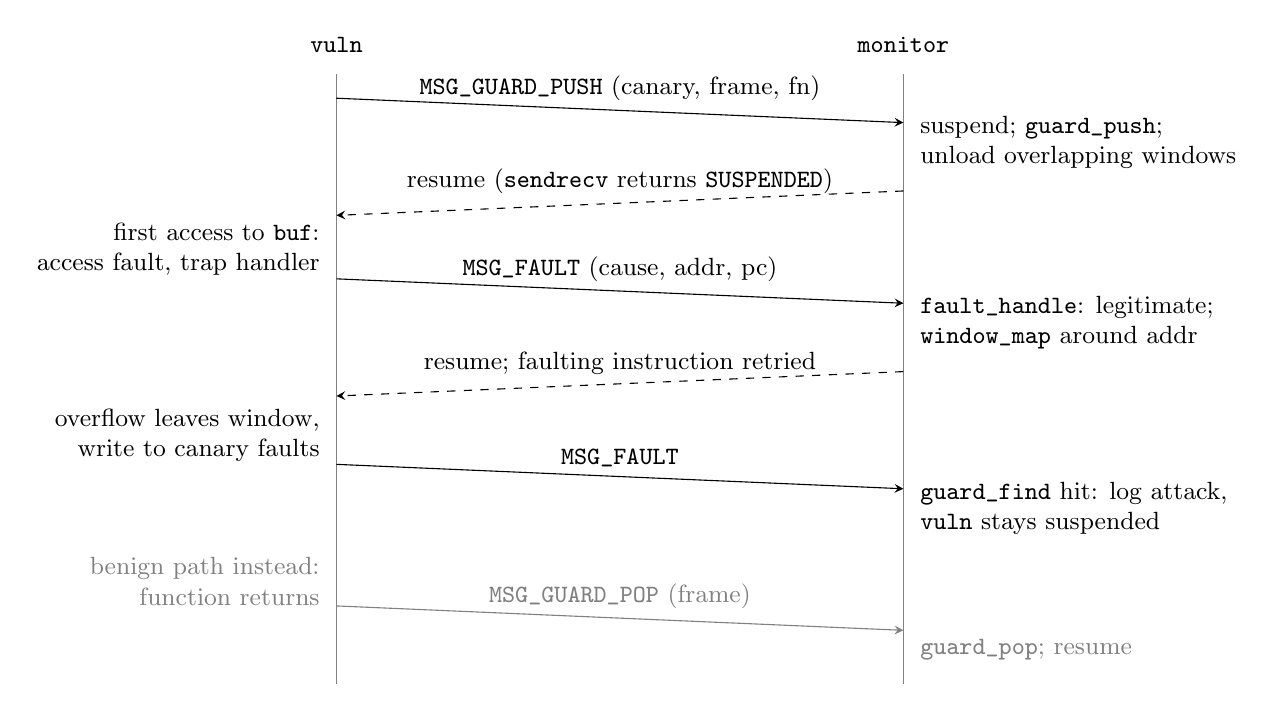
\begin{tikzpicture}[>=stealth, font=\small, x=0.9cm, y=0.62cm]
  \node[font=\small\bfseries] at (0,0.6) {\code{vuln}};
  \node[font=\small\bfseries] at (8,0.6) {\code{monitor}};
  \draw[gray] (0,0) -- (0,-12.5);
  \draw[gray] (8,0) -- (8,-12.5);
  \draw[->] (0,-0.5) -- node[above] {\code{MSG_GUARD_PUSH} (canary, frame, fn)} (8,-1);
  \node[right, align=left] at (8.1,-1.4) {suspend; \code{guard_push};\\unload overlapping windows};
  \draw[->,dashed] (8,-2.4) -- node[above] {resume (\code{sendrecv} returns \code{SUSPENDED})} (0,-2.9);
  \node[left, align=right] at (-0.1,-3.6) {first access to \code{buf}:\\access fault, trap handler};
  \draw[->] (0,-4.2) -- node[above] {\code{MSG_FAULT} (cause, addr, pc)} (8,-4.7);
  \node[right, align=left] at (8.1,-5.1) {\code{fault_handle}: legitimate;\\\code{window_map} around addr};
  \draw[->,dashed] (8,-6.1) -- node[above] {resume; faulting instruction retried} (0,-6.6);
  \node[left, align=right] at (-0.1,-7.4) {overflow leaves window,\\write to canary faults};
  \draw[->] (0,-8.0) -- node[above] {\code{MSG_FAULT}} (8,-8.5);
  \node[right, align=left] at (8.1,-8.9) {\code{guard_find} hit: log attack,\\\code{vuln} stays suspended};
  \node[left, align=right, text=gray] at (-0.1,-10.4) {benign path instead:\\function returns};
  \draw[->,gray] (0,-10.9) -- node[above] {\code{MSG_GUARD_POP} (frame)} (8,-11.4);
  \node[right, align=left, text=gray] at (8.1,-11.8) {\code{guard_pop}; resume};
\end{tikzpicture}
\caption{Lifecycle of a guarded stack frame. Every message blocks \code{vuln} until the monitor resumes it.}
\label{fig:lifecycle}
\end{figure}

\subsection{Design choices and rejected alternatives}

\paragraph{Guards in addition to canaries.}
A canary alone detects a linear overwrite when the function returns, after
the saved \code{ra} has already been replaced, and the response
(\code{__stack_chk_fail}) runs inside the compromised process. It misses
writes that skip the canary, and it fails if the canary is leaked. We keep
the canaries as the baseline and add guards that stop the first access to
the canary or the saved return state, before anything is overwritten, with
the response handled by an isolated process.

\paragraph{Per-frame guards instead of one stack guard.}
A single unmapped region below the stack only catches stack exhaustion. To
catch an overflow inside the stack, every live frame needs its own guards. We
register two per frame: \code{[canary, canary+8)} and the saved
\code{ra}/\code{s0} at \code{[frame-16, frame)}.

\paragraph{Living with eight PMP entries.}
Two entries are permanent (image and UART), which leaves six for the stack. A
heap-protection project on S3K rejected guard pages for this reason. We
avoid the limit by inverting the question: guards are not PMP entries at all.
The guard table is ordinary monitor memory (64 frames, 128 guards, in the
evaluated build), and the six PMP entries only describe which guard-free
windows are currently mapped. When all six are in use, the monitor evicts one
round-robin. Running out of PMP entries therefore costs extra faults, not
protection.

\paragraph{A separate monitor.}
The guard table and the PMP configuration must be out of reach of the
attacker. S3K only lets a process change another process's PMP through a
monitor capability, so the monitor is a separate process with a monitor
capability over \code{vuln}, and \code{vuln} holds no capability that could
change its own stack mappings.

\subsection{Compiler-generated stack canaries}

Both the kernel and every application are built with
\code{-fstack-protector-strong}. Each provides its own
\code{__stack_chk_guard} and \code{__stack_chk_fail}. The kernel seeds its
guard in \code{stack_chk_guard_init}, which \code{head.S} calls after
clearing \code{.bss} and before \code{kernel_init}; the function is compiled
without a stack protector because it changes the value it would check. The
seed mixes the timer, the guard's own address and the hart ID, then applies
the MurmurHash3 finalizer (multiplication by \code{0xff51afd7ed558ccd} and a
33-bit xor-shift). Applications call \code{util_stack_protect_init} first in
\code{main}, which does the same with \code{s3k_get_time}. In both cases the
lowest byte is cleared, so a string copy that stops at a NUL byte cannot
reproduce the canary.

Figure~\ref{fig:frame} shows the frame GCC 15.1 generates for \code{greet}
in the protected build. The 128-byte buffer starts at \code{sp+8} and ends
exactly at the canary, so the canary is the first thing a linear overflow
reaches. The callee-saved \code{s1} sits between the canary and \code{s0},
so the distance from the canary to \code{ra} depends on how many registers a
function saves. The guards therefore cannot assume a fixed canary offset.

\begin{figure}[htbp]
\centering
\small
\begin{tabular}{@{}rll@{}}
\toprule
Offset & Contents & Guard \\
\midrule
\code{sp+168} & saved \code{ra} & return guard \code{[frame-16, frame)} \\
\code{sp+160} & saved \code{s0} & return guard \\
\code{sp+152} & saved \code{s1} & --- \\
\code{sp+136} & canary (\code{sd a5,136(sp)}) & canary guard \code{[canary, canary+8)} \\
\code{sp+8} & \code{char name[128]} & mapped on demand \\
\bottomrule
\end{tabular}
\caption{Stack frame of \code{greet} (176 bytes, frame = \code{sp+176}) in the protected build, read from the disassembly of \code{vuln.elf}.}
\label{fig:frame}
\end{figure}

A canary mismatch ends in \code{__stack_chk_fail}. The kernel version prints
a message and halts the hart in a \code{wfi} loop. The application version
prints \code{*** stack smashing detected ***} and spins forever. Spinning is
not termination: the process keeps its time slice and capabilities. In the
full design this matters less, because an overflow faults on the guard before
the canary check is ever reached, and the monitor suspends \code{vuln}.

\subsection{Virtualized PMP stack guards}

\paragraph{Frame registration.}
\code{vuln} is compiled with \code{-finstrument-functions}, so GCC calls
\code{__cyg_profile_func_enter} after every prologue and
\code{__cyg_profile_func_exit} before every epilogue. The canary is always
written before the enter hook runs, so registering the guard never interferes
with the prologue. The enter hook is a short assembly preamble that captures
the stack pointer of the instrumented function before the hook opens its own
frame. The C part adds the function's frame size, taken from a table that the
build derives from the \code{-fstack-usage} output, to get the top of the
frame, locates the canary, and sends \code{MSG_GUARD_PUSH}. The exit hook sends
\code{MSG_GUARD_POP}. At \code{-Os}, GCC tail-calls the exit hook after the
canary check, so the epilogue would read the canary while its guard is still
registered, and every normal return would be reported as an attack.
\code{vuln} is therefore built with \code{-fno-optimize-sibling-calls}, which
moves the exit hook before the canary load in the epilogue.
\draftnote{Agaton: confirm how the hook locates the canary and frame
(\code{stack_usage.c}).}

\paragraph{Resume is the reply.}
S3K only lets a monitor change the PMP of a process that is suspended. A
process blocked in IPC is not enough: \code{s3k_mon_pmp_unload} on it
returns \code{S3K_ERR_INVALID_STATE}. The monitor therefore never sends a
reply message. \code{vuln} calls \code{s3k_sock_sendrecv} and blocks; the
monitor receives the message, suspends \code{vuln}, updates the guard table
and the PMP, and resumes it. \code{vuln}'s \code{sendrecv} then returns
\code{S3K_ERR_SUSPENDED}, which means the request is done. On an attack, the
monitor does not resume \code{vuln}. The socket is \code{S3K_IPC_NOYIELD}:
with \code{S3K_IPC_YIELD}, the waiting client timed out at the end of its time
slice and ran on before the monitor had finished.

\paragraph{Trap handler.}
The handler lives in a \code{.trap.text} section that the linker script
places at \code{0x80037000}, and its 2 KiB trap stack ends at
\code{0x80038000}. Both are inside the permanent image mapping, so the
handler can never fault on its own stack. It is marked
\code{no_instrument_function} so it does not send frame events, and
\code{used} so link-time optimization cannot drop it. It sends
\code{MSG_FAULT} with \code{ECAUSE}, \code{EVAL} and \code{EPC}, retries while
the monitor is not yet receiving, and returns. Returning restores
\code{EPC}, which points at the faulting instruction, so once a window is
mapped the instruction runs again and succeeds.

\paragraph{Fault classification.}
\code{fault_handle} applies the checks in order and stops at the first match:
\begin{enumerate}
  \item A cause other than an instruction, load or store access fault
  (\code{ECAUSE} 1, 5, 7) is a crash.
  \item An instruction fetch from the stack is an attack. Windows are
  read-write only, so stack shellcode can never run.
  \item An address inside a registered guard is an attack. The log names the
  guard kind and the owning function.
  \item An address outside \code{[0x8003F000, 0x80040000)} is out of bounds,
  which covers both stack exhaustion and a write past the top of the stack.
  \item The same \code{(EVAL, EPC)} pair twice in a row is a fault loop.
  \item Otherwise the access is legitimate: the monitor maps a window and
  resumes \code{vuln}.
\end{enumerate}
Every stop logs the reason, cause, address and program counter and leaves
\code{vuln} suspended.

\paragraph{Window mapping and invalidation.}
\code{window_map} searches from the whole 4 KiB stack downward in powers of
two for the largest NAPOT block that contains the faulting address, lies
inside the stack and overlaps no guard. A buffer that ends at its canary and
is aligned to its size is covered by a single window. The monitor derives a
PMP capability for that block from its memory capability over the stack,
moves it into \code{vuln}'s capability table, and loads it into a free slot
between 2 and 7, evicting one round-robin if all six are in use. Eviction
moves the capability back and deletes it. When a new guard is registered,
every loaded window that overlaps it is evicted, so no window ever covers a
live guard.

\paragraph{Implementation status.}
\draftnote{Replace \code{<commit>} with the evaluated commit, and confirm
that every component above is in it. At \code{ab70873} plus the uncommitted
\code{windows.c}/\code{faults.c} work, the enter and exit hooks still send
\code{(function, caller, sp)} instead of \code{(canary, frame, function)},
so the monitor registers the wrong addresses and guards are not enforced.}

\section{Evaluation}
\label{sec:evaluation}

\subsection{Experimental setup}

All runs use the \code{qemu_virt} platform (one hart) on QEMU 8.2.2 with
\code{-icount 3}, inside the project's \code{s3k-dev} container. The code is
compiled with GCC 15.1.0 for \code{rv64imac} with \code{-Os -g3
-fstack-protector-strong -fstack-usage}, and \code{vuln} additionally with
\code{-finstrument-functions -fno-optimize-sibling-calls}. \code{-flto} is disabled, because it breaks
\code{-fstack-usage}. The unprotected build is the same tree with
\code{-fno-stack-protector} in \code{projects/build.mk}. Every frame offset
below is read from the disassembly of the tested \code{vuln.elf}, not from
earlier notes. The input is sent over the UART. The suspension experiment is
\code{projects/test.07.ipc-suspend-reply}.
\draftnote{Add the evaluated commit hash.}

\subsection{Baseline results}

In the unprotected build, \code{greet} opens a 144-byte frame with the buffer
at \code{sp+0} and \code{ra} at \code{sp+136}. The target \code{win} is at
\code{0x80030082}, whose second byte is zero, so a full address cannot pass
through \code{alt_gets}. The saved \code{ra} is \code{0x80030176}, the
return point in \code{main}, which already has the same upper bytes. The
exploit sends 136 bytes of padding followed by \code{0x82}, and
\code{alt_gets} writes the terminating NUL into the second byte. The return
address becomes \code{0x80030082}, and the run prints
\code{You exploited the binary!}. The exploit reads the padding, the target
and the original return address from the ELF, and picks the shortest such
partial overwrite.

\begin{table}[htbp]
\centering
\small
\begin{tabularx}{\linewidth}{@{}p{0.30\linewidth}X@{}}
\toprule
Test & Observed result \\
\midrule
Benign input, protected build & Both prompts answered and returned normally. \\
Unprotected build, 136 bytes + \code{0x82} & Return redirected to \code{win}; \code{You exploited the binary!} printed. \\
Protected build, 136 \code{A} (canary overwritten) & \code{*** stack smashing detected ***}; \code{vuln} spins in \code{__stack_chk_fail}. \\
Protected build, 200 \code{A} (past stack top) & Monitor: \code{out of bounds cause:7 addr:80040000 pc:80030E1C}; \code{vuln} left suspended. \\
PMP unload while client blocked & \code{S3K_ERR_INVALID_STATE} in 10 of 10 rounds. \\
PMP unload/load while suspended & Success in 10 of 10 rounds; client's \code{sendrecv} returned \code{S3K_ERR_SUSPENDED}. \\
\bottomrule
\end{tabularx}
\caption{Baseline and infrastructure results.}
\label{tab:baseline}
\end{table}

The 200-byte run shows the bounds check working in practice. \code{greet}'s
buffer is the last frame before the top of the stack, so the overflow reaches
\code{0x80040000}. No PMP entry covers that address, the store inside
\code{alt_gets} faults, and the monitor stops \code{vuln} before the write
happens. In the 136-byte run, the input fills the 128-byte buffer and
overwrites all eight bytes of the canary; the terminating NUL lands in the
padding below \code{s1}. The epilogue's comparison fails and calls
\code{__stack_chk_fail}, which prints its diagnostic. Attaching GDB afterwards
shows \code{vuln}'s program counter at \code{0x80030a9e}, the infinite loop
at the end of \code{__stack_chk_fail}, and \code{vuln} still runnable: the
canary detected the overflow, but the process was not stopped. With 128 bytes,
the NUL only overwrites the canary's low byte, which is already zero, and the
function returns normally.
\draftnote{Rerun the 200-byte case on the final commit; the program counter
in the log line may move.}

\subsection{Attack matrix}

Each attack runs against the canary-only build and the full design.
Table~\ref{tab:matrix} gives the expected outcome from the design next to
the observed one.

\begin{table}[htbp]
\centering
\small
\begin{tabularx}{\linewidth}{@{}p{0.30\linewidth}XXX@{}}
\toprule
Attack & Expected, canary only & Expected, full design & Observed (canary / full) \\
\midrule
Linear overflow into \code{ra} & caught at return & stopped at first guard write & \resultplaceholder \\
Leak canary, write it back & missed & stopped: the read faults & \resultplaceholder \\
Indexed write skipping the canary & missed & stopped: return guard & \resultplaceholder \\
Overflow through pointer to a frame further up & caught at return & stopped: every frame guarded & \resultplaceholder \\
Shellcode on the stack & runs & stopped: windows are not executable & \resultplaceholder \\
Deep recursion & missed & stopped: bounds check & \resultplaceholder \\
\bottomrule
\end{tabularx}
\caption{Attack matrix.}
\label{tab:matrix}
\end{table}

\draftnote{Run each row and fill in the last column with the monitor's log
line or the canary diagnostic. Separate observed results from expectations
in the discussion below the table.}

\paragraph{Cost and validity.}
Performance was not a goal and was not measured. The cost of the design is
one IPC round trip for every function call and return, and one more for every
fault that maps a window.
\draftnote{Optionally report faults per call for \code{greet}.}
All results come from QEMU, not real hardware, and from a small test
application with two vulnerable functions.

\section{Why the Design Counters the Attacks}
\label{sec:why}

\paragraph{Linear overflow.}
A write that runs off the end of a buffer leaves the window that covers the
buffer. The next address is the canary, which is a guard and is never mapped,
so the store faults and \code{guard_find} identifies it. Nothing past the
window is written, so the saved \code{ra} is intact when \code{vuln} is
stopped. The canary remains as a second line of defense.

\paragraph{Writes that skip the canary.}
An indexed write that jumps over the canary lands on the saved \code{s0} or
\code{ra}, both inside the return guard \code{[frame-16, frame)}. This is the
case a canary cannot detect.

\paragraph{Canary disclosure.}
Guards are never mapped for reading either, so the attacker cannot read the
canary in order to write it back. The protection no longer depends on the
canary's randomness, because the value cannot be read at all.

\paragraph{Frames further up.}
The guard table covers every live frame, not only the current one. An
overflow through a pointer to a buffer in a caller's frame hits that caller's
guards. Eviction does not weaken this, because guards are never mapped
regardless of how many windows are in use.

\paragraph{Shellcode and stack exhaustion.}
Windows are RW only, and a fetch from the stack is classified as an attack.
Stack growth below \code{0x8003F000}, or a write past \code{0x80040000}, hits
memory that is never mapped and is classified as out of bounds; the 200-byte
run in Table~\ref{tab:baseline} shows the second case.

\paragraph{Attacks on the protection itself.}
The guard table and the window logic live in the monitor's memory, which
\code{vuln} cannot access. \code{vuln}'s capabilities do not include any
memory capability over its stack or any monitor capability, so it cannot map
windows itself. Its only influence on the monitor is the messages it sends.

\paragraph{What is not stopped.}
Within the threat model, an attacker who never takes over control flow cannot
forge frame events, because the hooks only run at real function boundaries.
An attacker who does gain code execution by some other route could send
\code{MSG_GUARD_POP} for a frame to unguard it, or skip registration. The
image is mapped RWX, so a write primitive into \code{.data} or \code{.bss}
could also place code there. Overwrites of locals inside a frame are not
detected.

\section{Individual Contributions}
\label{sec:contributions}

\subsection{Oliver Marcusson}

\paragraph{Canary integration and experimental infrastructure.}
I added stack canary support to the kernel and the applications
(\code{f9ae9c4}): \code{-fstack-protector-strong} in the build, guard
initialization before \code{kernel_init} in \code{head.S}, and separate
kernel and application handlers. Initialization had to run before the first
protected function and be compiled without a protector itself, since it
changes the value it would otherwise check. I created the vulnerable
demonstration project (\code{050237d}), made \code{alt_gets} usable from a
terminal (\code{ad0c336}), and put the guest UART on a TCP socket
(\code{2973ec0}) so that the attack could be scripted. On top of that I wrote
the pwntools exploit (\code{b89cd91}), which reads the target address and the
\code{ra} offset from the ELF instead of hard-coding them, because every
change to \code{greet} moves the frame. Before this I set up the shared
project template and development container used by the group.

\paragraph{Shared interface and suspension experiment.}
I wrote the shared interface in \code{interface.h} and the
\code{test.07.ipc-suspend-reply} experiment (\code{d341680}). The design
depends on the monitor changing \code{vuln}'s PMP while \code{vuln} waits for
a reply, and I needed to know whether S3K allows that before anything else
was built. The experiment showed that it does not: a blocked process cannot
be reconfigured, a suspended one can, and the resume can itself serve as the
reply. It also showed that the socket must be non-yielding. This became the
``resume is the reply'' protocol.

\paragraph{Fault path.}
I implemented the memory layout with a stack that has no permanent PMP entry
and a pinned trap region (\code{ab70873}), the boot grants in \code{app0},
the monitor's main loop, the trap handler that forwards faults, and
\code{fault_handle} with its classification order and attack log. I also
ran the baseline experiments in Section~\ref{sec:evaluation}.
\draftnote{Add the attack-matrix work and its commits once done.}

\subsection{Agaton Pirander}
\draftnote{To be written by Agaton, in first person: the enter and exit hooks
and the assembly preamble capturing the caller's stack pointer
(\code{66367c1}, \code{5b910da}); the frame and guard tables with
\code{guard_push}, \code{guard_pop} and \code{guard_find} (\code{f88e39b});
the \code{-fstack-usage} frame-size table (\code{7531310}); window
selection, slot management and invalidation in \code{windows.c}.}

\draftnote{Include an AI-assistance disclosure if required by the course,
accurately describing its role and how the output was verified.}

\section{Limitations and Conclusion}
\label{sec:conclusion}

\subsection{Remaining limitations}

The canary seed is built from the timer and an address, which is
predictable and not cryptographically strong; in the full design this
matters less, since the guard does not rely on the canary being secret. The
application-level \code{__stack_chk_fail} spins instead of terminating. Only
\code{vuln} is protected by guards, and only functions that GCC instruments
have canaries. The monitor trusts the frame events, and the guard table has a
fixed capacity of 64 frames. Finally, the evaluation is limited to QEMU and
one small application.

\subsection{Conclusion and future work}

Stack canaries can be added to S3K with little effort, but they detect an
overflow only after it has happened, and only if the canary is neither
skipped nor leaked. Capability-controlled PMP closes most of that gap. By
treating the eight PMP entries as a cache over a guard table in a trusted
monitor, every live frame's canary and saved return state can be kept
unmapped at any call depth, and an overflow faults before it overwrites
them. The main constraint is S3K's rule that PMP can only be changed while
the target is suspended, which forces one blocking round trip per call,
return and window fault. Next steps are to make the failure handler terminate
the process, protect the image with separate RX and RW regions, measure the
fault and IPC overhead, and reduce the trust placed in frame events.

\begin{thebibliography}{9}
\small

\bibitem{diversity}
P. Larsen, A. Homescu, S. Brunthaler, and M. Franz,
``SoK: Automated Software Diversity,''
\emph{IEEE Symposium on Security and Privacy}, 2014.
doi: \href{https://doi.org/10.1109/SP.2014.25}{10.1109/SP.2014.25}.

\bibitem{patagonix}
L. Litty, H. A. Lagar-Cavilla, and D. Lie,
``Hypervisor Support for Identifying Covertly Executing Binaries,''
\emph{USENIX Security Symposium}, 2008.

\bibitem{cflat}
T. Abera et al.,
``C-FLAT: Control-Flow Attestation for Embedded Systems Software,''
\emph{ACM Conference on Computer and Communications Security}, 2016.
doi: \href{https://doi.org/10.1145/2976749.2978358}{10.1145/2976749.2978358}.

\bibitem{s3k}
S3K project repository, \code{agpira1/s3k}, branch \code{2024-sys-sec},
revision \code{ab70873}.
\href{https://github.com/agpira1/s3k/tree/ab70873}{Source snapshot},
accessed October 2026.
% Replace with the full hash of the commit actually evaluated.

\end{thebibliography}
\end{document}
